\section{实验设置}

\noindent\textbf{数据集选择} \quad 根据该领域此前最先进的噪声模型Noise Flow\cite{noiseflow}、FGNM\cite{co},该领域最为广泛使用的数据集为智能手机图像去噪数据集(Smartphone Image Denoising Dataset,SIDD)\cite{sidd},因此本文同样选择SIDD数据集来评估本文提出的方法的性能。SIDD数据集包含320个噪声干净RAW图像对,这些图像对在不同的ISO水平和照明条件下,由5个不同的智能手机拍摄,包含10个不同的场景。ISO水平的范围是50到10000。与此同时,该数据集提供了一个简化的ISP图像处理管道,用于将图像从RAW域渲染到sRGB域,如下图所示:

\begin{figure}[htbp]
	\centering
	\begin{subfigure}{0.48\linewidth}
		\centering
		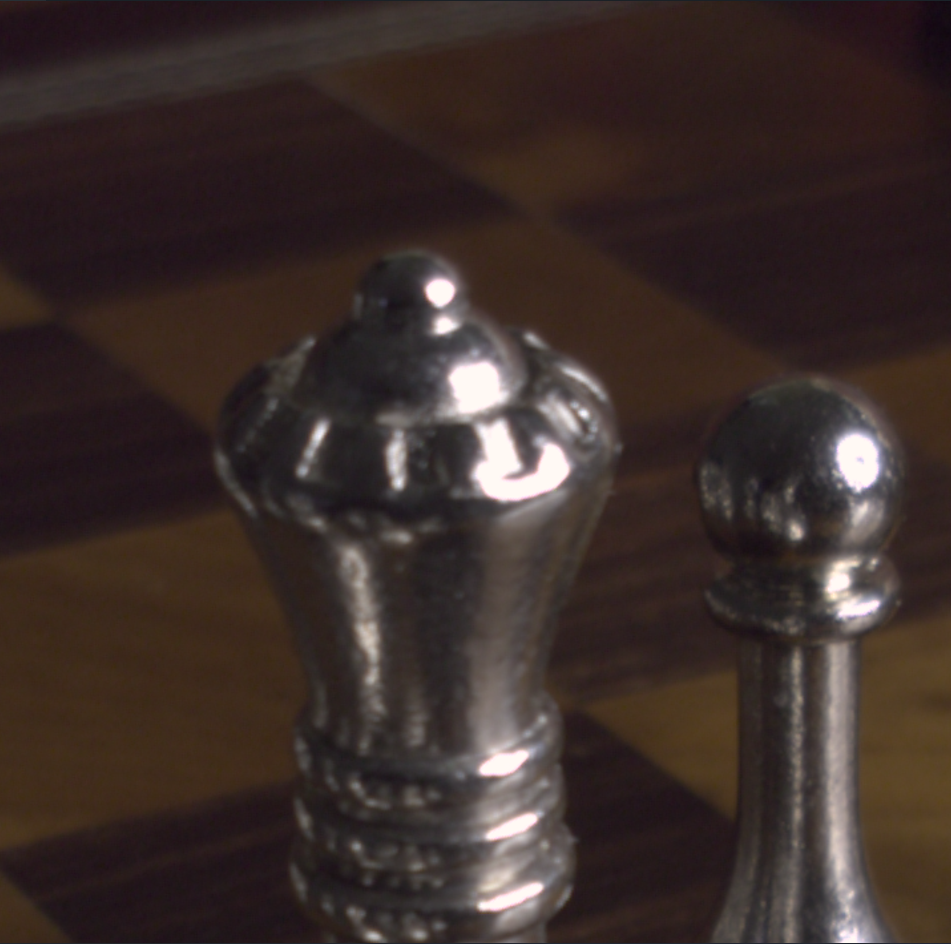
\includegraphics[width=\linewidth]{imgs/gtcut.png}
		\caption{干净图像}
		\label{gt}%文中引用该图片代号
	\end{subfigure}
	\centering
	\begin{subfigure}{0.4835\linewidth}
		\centering
		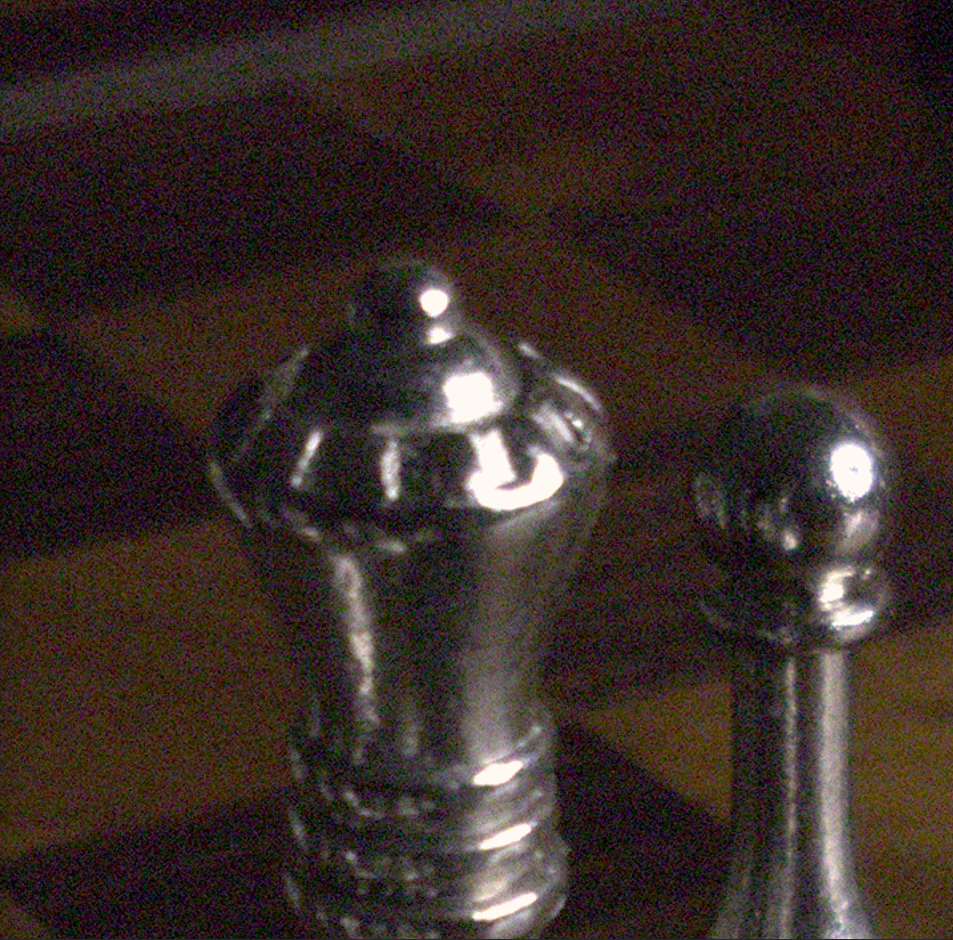
\includegraphics[width=\linewidth]{imgs/noisycut.png}
		\caption{噪声图像}
		\label{noisy}%文中引用该图片代号
	\end{subfigure}  
	
	\caption{SIDD中的干净-噪声图像对}
\end{figure}

在本文评估去噪性能的时候,还采用了极端低光去噪数据集(Extreme Low-light Denoising,ELD)\cite{eld}。ELD数据集包括10种不同的场景,由4种来自不同品牌的相机拍摄。该数据集选择了多种不同的拍摄设置,共产生了240个RAW图像对。

\begin{figure}[htbp]
	\centering
	\begin{subfigure}{0.49\linewidth}
		\centering
		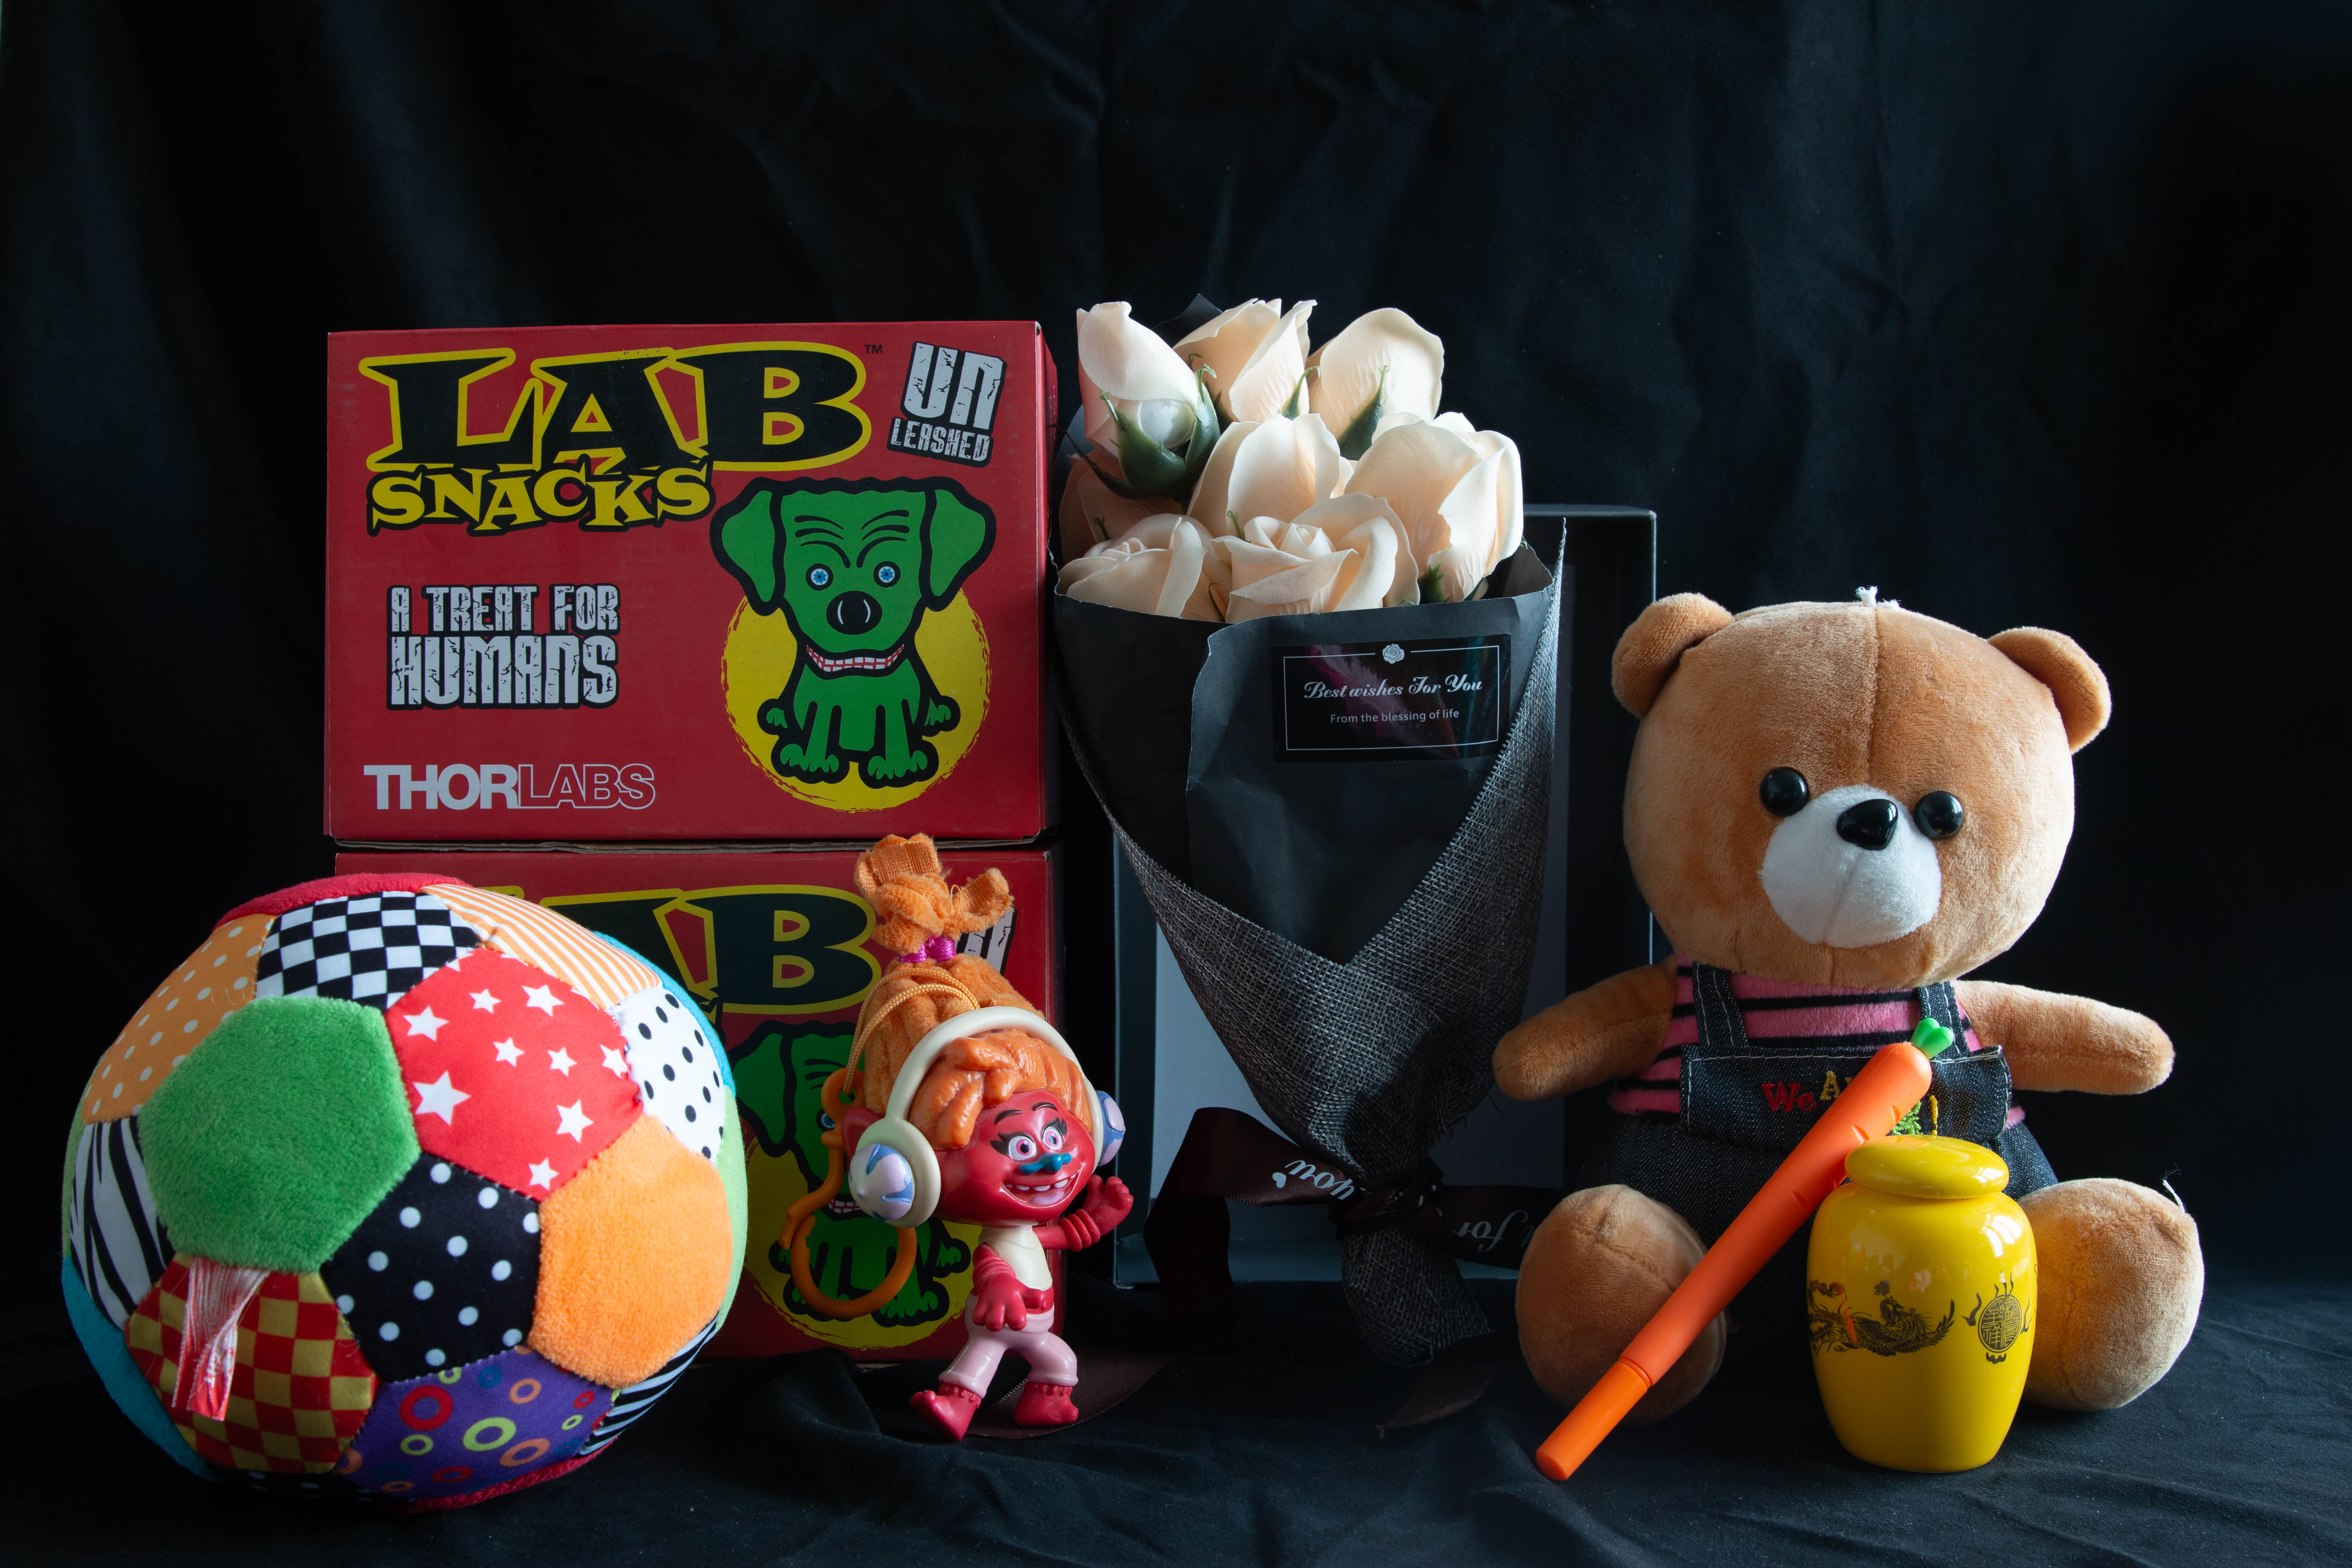
\includegraphics[width=\linewidth]{imgs/ELD1.jpg}
		
		\label{eld1}%文中引用该图片代号
	\end{subfigure}
	\centering
	\begin{subfigure}{0.49\linewidth}
		\centering
		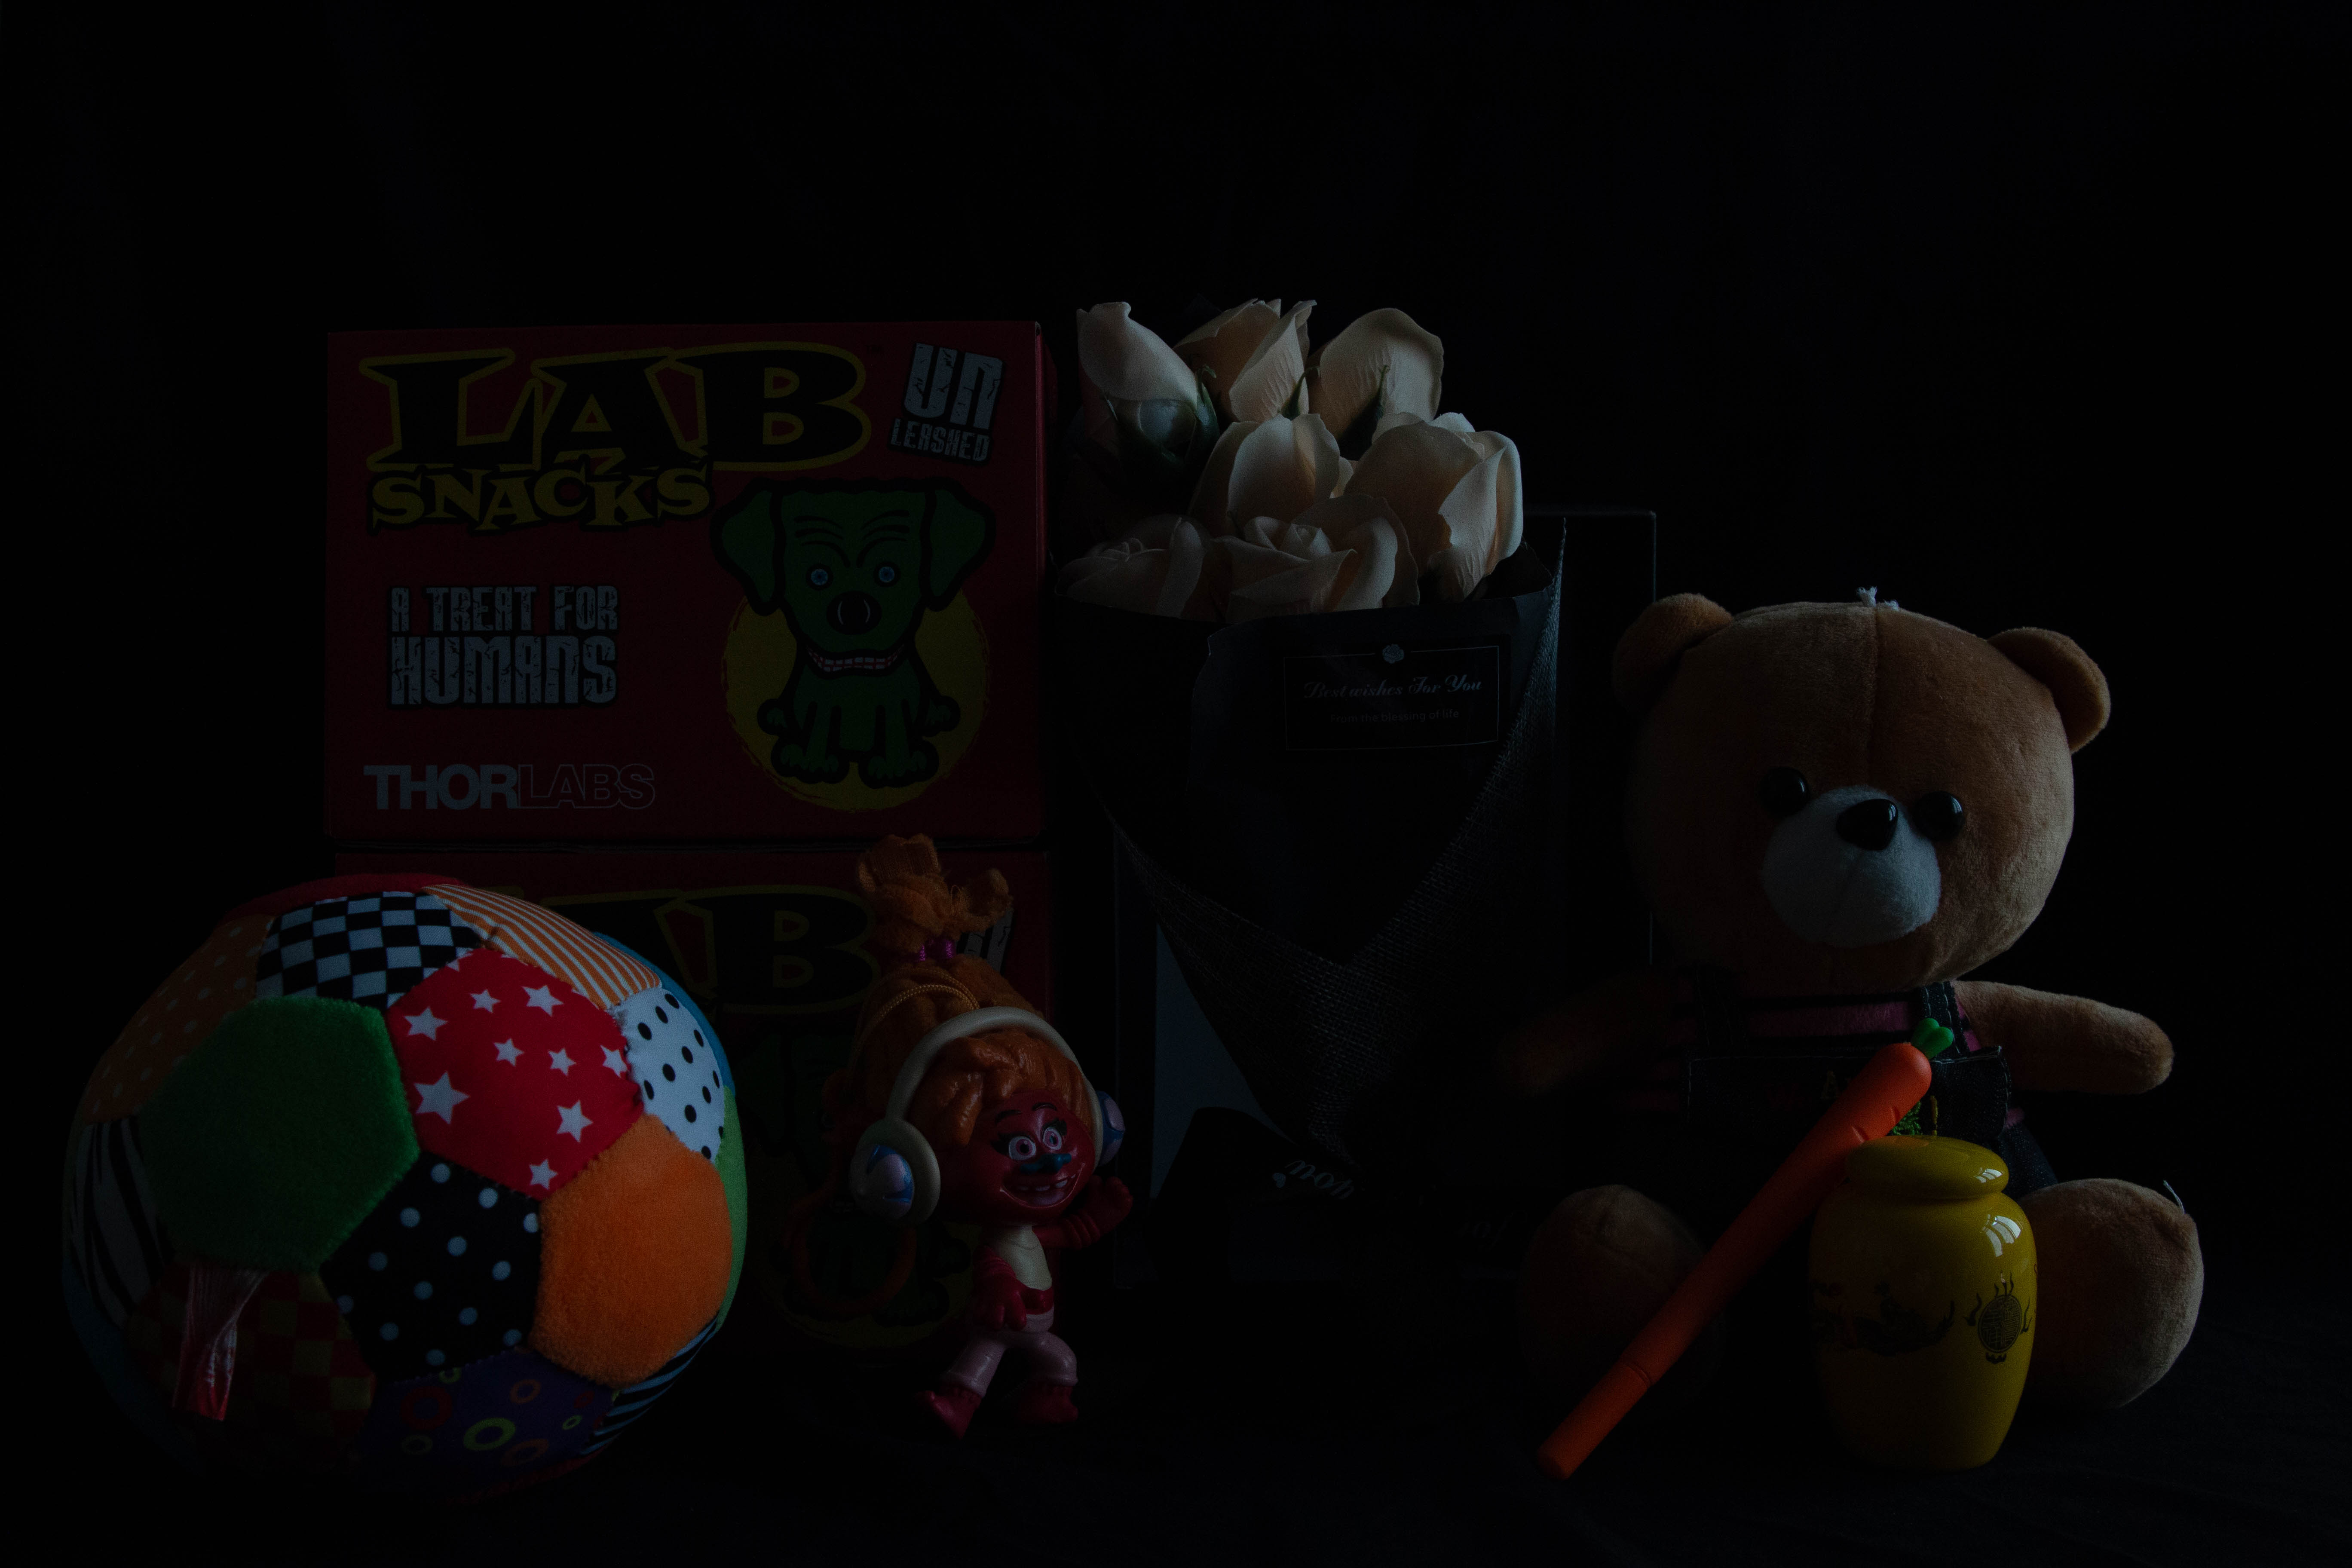
\includegraphics[width=\linewidth]{imgs/ELD3.jpg}
		
		\label{eld3}%文中引用该图片代号
	\end{subfigure}  
	
	\caption{ELD中同一场景下不同拍摄设置拍摄出的照片}
\end{figure}

\noindent\textbf{评估指标} \quad 为了定量评估性能,本文在对比时使用最常用的评估指标。对于噪声合成,为了评估合成噪声和真实捕获噪声之间的相似性,本文应用Kullback-Leibler (KL)散度来衡量两个分布之间的差异。KL散度的公式为:
\begin{equation}
	D_{K L}(p \| q)=\sum_{i=1}^n p(x) \log \frac{p(x)}{q(x)}
\end{equation}

对于真实去噪性能,本文使用峰值信噪比(Peak Signal-to-Noise Ratio,PSNR)作为指标之一,PSNR是基于均方误差(Mean Square Error,MSE)来定义的,给定一个大小为$m \times n$的原始图像$I$和经过处理的图像$K$,其MSE可定义为:
\begin{equation}
	M S E=\frac{1}{m n} \sum_{i=0}^{m-1} \sum_{j=0}^{n-1}[I(i, j)-K(i, j)]^2
\end{equation}
则PSNR可定义为:
\begin{equation}
	PSNR=20 \cdot \log _{10}\left(\frac{M A X_I}{\sqrt{M S E}}\right)
\end{equation}
其中$M A X_I$为图像的最大像素值。

此外,本文还使用结构相似性(Structural Similarity,SSIM)来作为两幅图像相似度的指标。SSIM由三个部分组成:亮度(luminance)、对比度(contrast)和结构(structure)。SSIM通过滑动窗口实现,遍历整张图像后将所有窗口的数值取平均值作为整张图像的SSIM指标。假设$x$、$y$分别表示两张图像窗口中的数据,亮度的计算公式为:
\begin{equation}
	l(x, y)=\frac{2 \mu_x \mu_y+c_1}{\mu_x^2+\mu_y^2+c_1}
\end{equation}
对比度的计算公式为:
\begin{equation}
	c(x, y)=\frac{2 \sigma_x \sigma_y+c_2}{\sigma_x^2+\sigma_y^2+c_2}
\end{equation}
结构的计算公式为:
\begin{equation}
	s(x, y)=\frac{\sigma_{x y}+c_3}{\sigma_x \sigma_y+c_3}
\end{equation}
其中$\mu$表示均值,$\sigma$表示方差,$c$表示常数,最后SSIM的计算公式为:
\begin{equation}
	SSIM(x, y)=\left[l(x, y)^\alpha \cdot c(x, y)^\beta \cdot s(x, y)^\gamma\right]
\end{equation}
参数$\alpha$、$\beta$、$\gamma$通常取1。

\noindent\textbf{数据增强} \quad 在现有噪声参数的基础上,本文采用了一种有价值的数据增强策略,即在参数中添加方差为$0.1$的高斯扰动。这项技术通过引入方差作为附加信息,丰富了有限的数据集,有助于提高生成模型的鲁棒性。数据集的这种微小但有意义的变化可以与本文预训练的标准化流模型无缝集成,展示了一种增强的噪声建模方法。此外,它还允许模型考虑不可预测的真实世界变化,从而提高了神经网络噪声建模能力的准确性和有效性。


\noindent\textbf{实现细节} \quad 本文的模型训练设置效仿了Noise Flow模型\cite{noiseflow},使用Adam优化器进行训练,迭代20万次。初始学习率为0.0002,学习率调整使用余弦退火算法。模型训练并不会使用整张图片,而是将图片切成$64\times 64$的块,同时一次迭代会处理16个样本。

\section{实验结果}



\subsection{噪声建模的对比}

为了评估所提出的噪声建模方法的噪声合成性能,本文将合成噪声和真实噪声之间的KL散度与几种最先进的噪声建模方法进行了比较。
\begin{table*}[htbp]
	\begin{center}
		\tabcolsep = 1.7cm
		\caption{不同噪声建模方法在SIDD数据集上的平均KL散度表现(越小越好)}
		\label{compareNoise}
		\begin{tabular}{c|c}
			\toprule[1.5pt]
			方法 & 平均KL散度\\
			\midrule [1pt]
			AWGN & 0.7544\\
			P-G \cite{foi2008noise} & 0.0467\\
			Noise Flow \cite{noiseflow} & 0.0590 \\
			CANGAN \cite{learningcamera} & 0.0220\\
			FGNM \cite{co}& 0.0211\\
			\midrule[1pt]
			本文的模型& \textbf{0.0188}\\
			
			\bottomrule[1.5pt]
		\end{tabular}
	\end{center}
\end{table*}

平均KL散度的比较如表\ref{compareNoise}所示。参与比较的基准方法包括参数化噪声模型(即加性高斯白噪声模型和泊松-高斯噪声模型\cite{foi2008noise})和基于深度学习的噪声模型(即Noise Flow\cite{noiseflow}、CANGAN\cite{learningcamera}和FGNM\cite{co})。

可以看到,在参数化噪声建模方法中,AWGN模型的性能最差,P-G噪声模型由于包含了信号依赖性,更适合于模拟真实噪声。深度学习方法Noise Flow\cite{noiseflow}由于其训练的不稳定性,性能略逊于P-G。本文提出的方法获得了最佳的KL散度表现,证明了优越性。

各种噪声建模方法合成噪声图像的比较如图\ref{fig:compareNoise}所示,图中展示了来自不同ISO水平(100到1600)和光照条件的样本(N:正常光,L:暗光)。

\begin{figure}[h]
	\centering
	\includegraphics[width=1.0\textwidth]{imgs/compareNoise.pdf}
	\caption{ISO水平和照明条件(N:正常光,L:暗光)显示在左侧,KL散度显示在图像块左上角,这些RAW图像块通过SIDD提供的ISP处理管线进行可视化}
	\label{fig:compareNoise}
\end{figure}

本文在图\ref{viscom1}和\ref{viscom2}中展示了SIDD数据集上的更多可视化结果。可以看出,本文的方法生成的噪声图像在视觉上比其他方法更接近于真实的噪声分布,KL散度也定量地证明了这点,体现了本文所提出的方法在噪声建模任务中的优越性。

\begin{figure}[htbp]
	\centering
	\begin{subfigure}{\linewidth}
		\centering
		\includegraphics[width=0.73\linewidth]{imgs/viscom1.pdf}
		\caption{}
		\label{viscom1}%文中引用该图片代号
	\end{subfigure}
	\centering
	\begin{subfigure}{\linewidth}
		\centering
		\includegraphics[width=0.73\linewidth]{imgs/viscom2.pdf}
		\caption{}
		\label{viscom2}%文中引用该图片代号
	\end{subfigure}  
	
	\caption{不同噪声模型合成的噪声图像对比}
\end{figure}

\subsection{真实图像去噪}

为了进一步证明所提出方法的噪声生成能力,本文使用不同的噪声建模方法来生成成对的噪声-干净样本并训练RAW图像去噪网络。通过评估真实噪声图像上的去噪性能,可以进一步比较噪声先验学习的准确性。采用Noise Flow\cite{noiseflow}的实验思路,本文使用在相关工作介绍过的的标准DnCNN网络\cite{dncnn}作为去噪网络,包含10个卷积层。

ELD数据集上的去噪结果如表\ref{dncnneld}所示,可以看出,以本文的模型作为噪声先验训练的DnCNN模型在PSNR和SSIM指标上取得了显著更高的性能。

\begin{table}[h]
	\centering
	\caption{对比不同噪声先验DnCNN以及盲去噪方法Nois2Noise在ELD数据集上的表现}
	\label{dncnneld}
	\begin{subtable}{\linewidth}
		\centering
		\caption{PSNR}
		\resizebox{\textwidth}{!}{
			\begin{tabular}{c|c|ccccc}
				\toprule[1.5pt]  
				相机型号 &  快门速度(s) & Gaussian  & P-G\cite{foi2008noise} &  Noise2Noise\cite{noise2noise} & 真实噪声 & 本文的模型 \\
				\midrule[1pt]  
				\multirow{2}{*}{Sony A7S2} & $1/400$ & 42.35 & 42.46 & 41.63 & 44.50 & \textbf{45.49} \\
				& $1/800$ & 38.93 & 38.88 & 37.98 & 42.45 & \textbf{43.37} \\
				\midrule[1pt]			               
				\multirow{2}{*}{Nikon D850} & $1/400$ & 39.57 & 40.29 & 40.47 & 41.28 & \textbf{42.17} \\
				& $1/800$ & 36.68 & 37.26 & 37.98 & 39.44 & \textbf{39.98}\\
				\midrule[1pt]
				\multirow{2}{*}{Canon EOS70D} &$1/400$& 40.59 & 40.94 & 38.21 & 41.10 &\textbf{ 41.17}\\
				&$1/800$& 37.49 & 37.64 & 34.33 & 37.32 & \textbf{38.26}\\
				\midrule[1pt]		                  
				\multirow{2}{*}{Canon EOS700D}&$1/400$& 39.77 & 40.08 & 38.29 & 39.05 & \textbf{40.07}\\
				&$1/800$& 37.67 & 37.86 & 34.94 & 36.50 & \textbf{37.56}\\
				\bottomrule[1.5pt]
			\end{tabular}
		}
	\end{subtable}
	
	\begin{subtable}{\linewidth}
		\centering
		\caption{SSIM}
		\resizebox{\textwidth}{!}{
			\begin{tabular}{c|c|ccccc}
				\toprule[1.5pt]  
				相机型号 &  快门速度(s) & Gaussian  & P-G\cite{foi2008noise} &  Noise2Noise\cite{noise2noise} & 真实噪声 & 本文的模型 \\
				\midrule[1pt]  
				\multirow{2}{*}{Sony A7S2} & $1/400$ & 0.893 & 0.889 & 0.856 & 0.971 & \textbf{0.982} \\
				& $1/800$ & 0.813 & 0.812 & 0.775 & 0.945 & \textbf{0.952} \\
				\midrule[1pt]			               
				\multirow{2}{*}{Nikon D850} & $1/400$ & 0.823 & 0.845 & 0.848 & 0.938 & \textbf{0.947}  \\
				& $1/800$ & 0.757 & 0.786 & 0.820 & \textbf{0.910} & 0.899 \\
				\midrule[1pt]
				\multirow{2}{*}{Canon EOS70D} &$1/400$& 0.925 & 0.934 & 0.826 & 0.931 & \textbf{0.947} \\
				&$1/800$& 0.871 & 0.873 & 0.704 & 0.867 & \textbf{0.895} \\
				\midrule[1pt]		                  
				\multirow{2}{*}{Canon EOS700D}&$1/400$& 0.884 & 0.897 & 0.859 & 0.906 & \textbf{0.913} \\
				&$1/800$& 0.870 & 0.879 & 0.766 & 0.850 & \textbf{0.896} \\
				\bottomrule[1.5pt]
			\end{tabular}
		}
	\end{subtable}
	
\end{table}

值得注意的是,本文的噪声建模方法提供了更多的训练样本,因此与真实噪声先验相比,以本文的模型作为噪声先验训练的DnCNN网络可以获得相似或更高的结果。

SIDD数据集上本文的模型表现仍然优异,表\ref{dncnnsidd}展示了PSNR指标的定量分析,图\ref{fig:dncnnsidd}展示了视觉效果的对比,本文的模型都取得了最好或仅次于真实噪声先验的效果。

\begin{table}[htbp]
	\begin{center}
		
		\caption{对比不同噪声先验DnCNN在SIDD数据集上的表现}
		\label{dncnnsidd}
		\begin{tabular}{c|cccc}
			\toprule[1.5pt]
			方法 & 400-L & 400-N & 800-L & 800-N \\
			\midrule[1pt]
			Gaussian & 43.79 & 52.20 & 56.59 & 49.94 \\
			Noise Flow\cite{noiseflow} & 47.79 & 56.03 & 56.64 & 50.72 \\
			DnCNN-Real & 44.21 & 57.94 & \textbf{57.10} & 49.41 \\
			\midrule[1pt]
			本文的模型 & \textbf{48.24} & \textbf{58.21} & 56.79 & \textbf{50.98} \\
			\bottomrule[1.5pt]
		\end{tabular}
	\end{center}
\end{table}

\begin{figure}[h]
	\centering
	\includegraphics[width=1.0\textwidth]{imgs/dncnnsidd.pdf}
	\caption{不同噪声先验的视觉去噪效果}
	\label{fig:dncnnsidd}
\end{figure}

\section{消融实验}

为了验证所提出方法的有效性,本文进行了两项消融研究。本文消融了预训练的噪声先验以及数据增强策略,消融结果如表\ref{ablation}所示。表中本文提出的基于流模型的噪声参数先验(Flow-based Parameter Prior)简称为FPP,数据增强(Data Augmentation)简称为DA。表中比较了不同变体的PSNR和SSIM结果,可以看到,在预训练了基于流的参数先验后,由于噪声建模更加精确,去噪结果得到了显著改善。数据增强策略也能带来更高的结果。

\begin{table}[h]
	\begin{center}
		\caption{消融实验的结果}
		\label{ablation}
		\begin{tabular}{cc|cc|cc|cc|cc}
			\toprule[1.5pt]
			\multirow{2}{*}{FPP} & \multirow{2}{*}{DA} & \multicolumn{2}{c|}{ Sony A7S2 } & \multicolumn{2}{c|}{ Nikon D850 } & \multicolumn{2}{c|}{ Canon EOS70D } & \multicolumn{2}{c}{ Canon EOS700D } \\
			& & 1/400 & 1/800 & 1/400 & 1/800 & 1/400 & 1/800 & 1/400 & 1/800 \\
			\midrule[1pt]
			
			\multirow{2}{*}{$\checkmark$} & & 45.10 & 42.53 & 41.93 & 38.10 & 40.06 & 37.99 & 39.37 & 36.02 \\
			& & 0.978 & 0.947 & 0.921 & 0.884 & 0.938 & 0.825 & 0.869 & 0.899 \\
			\midrule[1pt] 
			
			& \multirow{2}{*}{$\checkmark$} & 45.06 & 42.10 & 41.26 & 37.63 & 39.76 & 37.94 & 39.52 & 35.47 \\
			& & 0.974 & 0.938 & 0.932 & 0.874 & 0.919 & 0.825 & 0.886 & 0.875 \\
			\midrule[1pt] 
			
			\multirow{2}{*}{$\checkmark$} & \multirow{2}{*}{$\checkmark$} & 45.49 & 43.37 & 42.17 & 39.98 & 41.17 & 38.26 & 40.07 & 37.56 \\
			& & 0.982 & 0.952 & 0.947 & 0.899 & 0.947 & 0.895 & 0.913 & 0.896 \\
			\bottomrule[1.5pt]
		\end{tabular}
	\end{center}
\end{table}